\pdfinfoomitdate=1
\pdftrailerid{}
\documentclass[11pt]{article}
\usepackage[letterpaper,margin=18mm,top=22mm,bottom=20mm,headheight=15pt]{geometry}
\usepackage{tikz,fancyhdr,amsmath,amssymb,array,booktabs,hyperref,lmodern}
\usepackage[T1]{fontenc}
\hypersetup{hidelinks}\pagestyle{fancy}\fancyhf{}
\fancyhead[L]{\small Week 88 / Packing and kissing circles / Adult guide}
\fancyfoot[L]{\small Bellingham Math Circle / Week 88 / W88-FAC-v1}\fancyfoot[R]{\thepage}
\setlength{\parindent}{0pt}\setlength{\parskip}{6pt}
\newcommand{\heading}[1]{\par\textbf{#1}\par}
\begin{document}
\heading{Mathematical overview: what is true, and under which rules}
\textbf{Equal-disk kissing theorem.} In a plane, at most six nonoverlapping disks of radius $r>0$ can each touch a central disk of the same radius externally. Six fit. Their centers lie on a circle of radius $2r$. Two neighboring outside centers must be at least $2r$ apart, so their center rays need at least $60^\circ$ between them. Seven such gaps exceed one full turn. With six, all gaps are exactly $60^\circ$: every neighboring outside pair touches. This is a local ring theorem, not an infinite-plane density theorem or a tray-packing maximum.

\textbf{Different sizes.} Disks of radii $a,b$ do not overlap exactly when their center distance is at least $a+b$. Congruent radius-$r$ outside disks touching a radius-$R$ center need angular gaps at least $2\arcsin(r/(R+r))$. Thus the maximum ring size is
\[\left\lfloor\frac{\pi}{\arcsin(r/(R+r))}\right\rfloor.\]
For 40 mm outside / 80 mm center diameters the maximum is nine; reversing sizes gives four; twelve 40 mm disks fit around a 120 mm center. This formula assumes all outside disks have the same size. If both sizes must occur outside, the maxima are eight about the 80 mm center and five about the 40 mm center, by separate pair-angle bounds (page 6). Trigonometry is optional adult background, not an entry prerequisite.

\textbf{Finite trays.} Eleven 40 mm disks fit in a 160 mm wide tray with height $40+40\sqrt 3\approx 109.282$ mm, in straight horizontal rows of four, three and four. This is the minimum height \emph{for those three rows}: four-disk rows have forced horizontal positions, and each intervening row gap is at least $20\sqrt 3$ mm. Thus these rows fit an exact 110 mm tray and do not fit a 108 mm tray. No unrestricted finite-tray optimum is claimed. The practical 112 mm tray adds about 2.7 mm of height but no width: 160 mm is exactly four diameters, so disks wider than 40 mm cannot make a row of four in any of the trays.

\textbf{Discovery map.} Optional K--1 entry: touch, overlap and fitting; an adult can read and record. Grades 2--3: construct and improve rings/trays, count final pieces. Grades 4--5: use centers, equal lengths and a whole turn to prove six and its rigid equality case; later distinguish a row-constrained impossibility from an unrestricted claim. Unequal-size upper bounds and exact radicals are readiness-dependent adult conversations. An object or drawing argument is a proof when it covers every legal arrangement.

A successful construction proves a lower bound. Repeated unsuccessful attempts suggest a conjecture, not an upper bound. The geometric arguments prove the stated limits. All materials and timings remain unpiloted; physical printing, circle accuracy and fit have not been rehearsed.
\newpage
\heading{Preparation and a manageable first visit}
Per pair: thirteen rigid circular disks 40 mm across (mark one center), five disks 80 mm across (one may be the middle), a ruler, nonstretch thread and small center stickers. Each table also needs one 120 mm middle disk for Problem 11. A clear desk mat at least $260\times 260$ mm supports large and mixed rings; it is not a Letter-page cutout. A center mark may go on the back so the same piece can be used in a tray.

For the eleven children at three fixed tables (K, K, 1, 1; four third graders; 4, 4, 5), prepare five kits: two pairs at each four-child table, one kit for the upper trio. Total: 65 small and 25 large disks and three 120 mm middles. Upper roles rotate among builder, checker and recorder. Every table has one anchored adult; the younger table's adult need not teach the angular proof. The family may instead serve selected tables with a familiar previously prepared activity at the others.

\textbf{Where the disks come from.} Either buy laser-cut circles 40, 80 and 120 mm across (wood, acrylic or card craft blanks are sold in metric sizes; avoid 1.5-inch circles, which are 38.1 mm), or print the three materials pages on card stock at Actual Size and cut on the lines. For five kits print materials page 1 five times, page 2 twice and page 3 three times: 26 large, 69 small and three 120 mm disks. Cutting is roughly a minute a disk (untested estimate); the disks are reusable.

\textbf{How exact the disks must be.} Ring answers depend only on size ratios: every ring maximum (Problems 1, 3--6, 10, 11) stays the same if each disk is up to 0.5 mm under its printed size and none is over. Six disks around the printed 40 mm middles then leave a gap of at most about 1.7 mm in all; outside disks larger than the middle make the six press. The trays need more: four disks fill the 160 mm width only if each is at most 40.0 mm, and Problem 8's answer changes for disks under 39.63 mm (1.5-inch circles fit the 4--3--4 rows in 102.6 mm). Use disks measured at 39.7--40.0 mm for Problems 7--9, or treat those trays as center-distance drawings.

Print student pages single-sided US Letter, Actual Size. For a first visit print pages 1--2, one copy per pair; for the Grades 4--5 trio print pages 1--5, with Problem 6 as the target. Offer page 3 for changed-size rings and page 4 for mixed rings only when wanted. Page 5 introduces centers; pages 6--7 are exact-tray continuations; page 8 contains optional upper-bound investigations. These are choices over several visits, not an eight-page hour. Keep one whiteboard available to save a construction without requiring each child to copy it.

\textbf{Before classroom use: still untested.} Measure disks in perpendicular directions. Measure each printed tray's clear interior: $160\times 112$, $160\times 110$, $160\times 108$ mm. Boundary ink lies outside the interior. Verify that six equal neighbors fit around the center and that pieces slide without curled edges or raised stickers interfering. The 110 mm eleven-disk construction has only $0.718$ mm vertical spare room; do not use imperfect cutouts to declare it impossible. Use measured rigid disks for play, or treat the tight tray as an ideal center-distance drawing. Never relabel a physical 112 mm fit as 110 mm. Preparation estimate with reusable disks: 20--35 minutes; cut a printed kit once and keep it, rather than cutting circles each week.

\textbf{Launch together.} After five minutes of movement, allow two minutes handling disks. Put down one center disk, one touching disk, one overlapping disk and one separated disk. Ask a child to show which outside disk obeys the ring rule; let a partner check. Say: ``Every outside piece touches this one. Pieces can touch each other, but cannot cover each other.'' Stop before completing a ring. Children then choose placements themselves. For a tray route demonstrate putting a disk wholly inside its border; central contact is no longer required.

Allow 25--35 minutes on Problem 1 or 2, with changed sizes only if useful; the upper trio can move on to Problems 3--6 once they have a six-ring. A child who cannot retain tangency can continue tray fitting; adult reading is appropriate, adult choice of every placement is not. Share one construction or one reason a claimed bound is convincing. Revisit the same materials later for centers and equality, then mixed sizes or tray sensitivity. Finishing every page is not the goal.
\newpage
\heading{Concrete solutions: Problems 1--5}
\textbf{1. Equal rings.} Six outside disks fit. Place their centers every $60^\circ$ on a circle of radius 40 mm about the center. Neighbor center distances are 40 mm. A child can find a good ring and stop; defer the upper bound to Problem 6. Hints in order: let the outer pieces touch one another; hold one in place while moving its neighbors. If a child claims seven, ask the partner to check every contact and overlap. Physical near-contact is not exact tangency.

\textbf{2. Practical tray.} The requested maximum hunt is an investigation; this guide proves an eleven-disk construction, not that eleven is the unrestricted maximum. A nine- or ten-disk improvement is worthwhile. A square-grid baseline holds eight (four in each of two rows). Eleven fit by staggering three between two rows of four. In millimetres from the lower-left corner, use
\[
\begin{array}{c|c}
y&x\\\hline
20&20,60,100,140\\
20+20\sqrt 3&40,80,120\\
20+40\sqrt 3&20,60,100,140
\end{array}
\]
The height is about 109.282 mm, so the 112 mm tray has about 2.718 mm extra height. Hints: compare gaps between two touching disks with the gap directly above a disk; move a whole row. Do not claim a global optimum from the number of available pieces or from failed attempts.

\textbf{3. Small disks about a large center.} Nine fit: outer centers at radius 60 mm, equally spaced at $40^\circ$. Neighbor distance $120\sin 20^\circ\approx 41.04$ mm exceeds 40. Ten would require more than a full turn; see page 6. Hints: keep each small disk touching the large center while sliding; check the last gap before counting the ring. A legal eight-disk construction remains valid evidence, even if not best.

\textbf{4. Large disks about a small center.} Four fit at right angles with outer-center radius 60 mm. Neighbor distance $60\sqrt 2\approx 84.85$ mm exceeds 80. Five are impossible by the angular bound. The outer-center radius is 60 in both Problems 3 and 4, but the outside pieces differ. Ask which disk-to-disk clearance changed. This contrast is accessible without inverse trigonometry.

\textbf{5. Mixed outside sizes.} Both sizes must occur among the outside disks, independently of the middle size. Around the large center, an eight-piece witness uses one large neighbor at angle 0 and seven small ones at angles 50,90,130,170,210,250,290 degrees. Around the small center, a five-piece witness uses one large at 0 and four small at 80,140,200,260 degrees. All touch the center and all pairs avoid overlap; page 6 proves the maxima.

Do not begin with those witnesses. A concrete hint is to make a legal same-size ring, replace one outside piece by the other size along the same center ray, then repair any overlap. Around either middle a large disk takes more of the turn than a small one: putting a large disk in place of a small one between two small ones takes about $18.5^\circ$ more around the 80 mm middle and about $21^\circ$ more around the 40 mm middle. Allow 15--30 minutes for mixed exploration or another visit. The guide's exact counts are adult answers, not compulsory proof targets for younger children.
\newpage
\heading{Problem 6: why six, and why every neighbor touches}
Use the student page's unequal-radius bridge first: two touching disks, join their centers through the contact point, then combine the two radii. It explains what a center-distance diagram records without supplying the six-ring answer. Let children put stickers on centers and use thread between them. For equal 40 mm disks, each outside center is 40 mm from the middle center.

Choose two consecutive outer centers $A,B$ and middle center $O$. The two radii $OA,OB$ are 40 mm. Nonoverlap means $AB\ge 40$ mm. When $AB=40$ the triangle is equilateral. Its angle at $O$ is $60^\circ$. Moving the two fixed-length radii closer makes their endpoint distance smaller, hence creates overlap. Therefore each circular gap is at least $60^\circ$; a gap larger than a half-turn certainly also meets this lower bound.

\begin{center}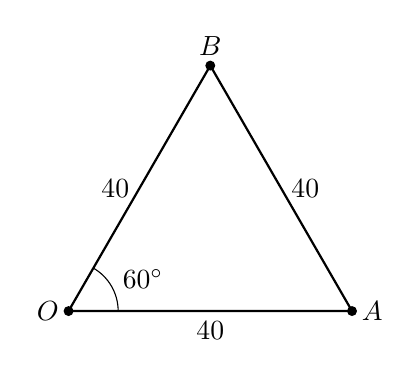
\begin{tikzpicture}[scale=0.9]
\coordinate(O)at(0,0);\coordinate(A)at(4,0);\coordinate(B)at(2,3.464);
\draw[thick](O)--node[below]{40}(A)--node[right]{40}(B)--node[left]{40}(O);
\foreach \p in {O,A,B}{\fill(\p)circle(2pt);}
\node[left]at(O){$O$};\node[right]at(A){$A$};\node[above]at(B){$B$};
\draw(0.7,0)arc(0:60:.7);\node at(1.05,.45){$60^\circ$};
\end{tikzpicture}\end{center}
This is the \emph{least-gap} triangle. Do not say all nonoverlapping neighbors always make an equilateral triangle: their separation may be larger.

Seven successive gaps would require at least $7\cdot 60=420^\circ$, but going once around the center gives $360^\circ$. The six-piece construction proves attainability. For equality, six gaps each at least 60 sum to 360, so all six equal 60. Every outside neighbor pair therefore touches. A visible physical gap in a nominal six-ring calls for checking disk accuracy and actual central contacts, not abandoning the ideal theorem.

\textbf{Hints, as needed.} First ask what center distance would be too short. Next hold two 40 mm thread radii at $O$ and bring their endpoints closer. Then compare a whole turn with equal equilateral-triangle wedges. An adult can make six congruent 60-degree wedges on blank paper, or use six green pattern-block triangles; a seventh cannot fit around one vertex. No child needs a protractor computation to explain the obstruction. Allow a full return visit for this shift from making to certifying.

\textbf{Further concrete contrast.} Five disks have flexible arrangements: delete one from the six-ring (four 60-degree gaps and one 120-degree gap), or place five evenly (five 72-degree gaps). These differ even after rotating the entire ring. This optional adult question shows why rigidity belongs to the sharp bound; it preserves the reserved plan's five-neighbor comparison without interrupting the main student question.
\newpage
\heading{Problems 7--9: a construction and its exact limit}
\textbf{7. Eleven disks in the 110 mm tray.} Use the coordinates on page 3. Nearest centers in adjacent rows have horizontal difference 20 and vertical difference $20\sqrt 3$, so squared distance is $20^2+(20\sqrt 3)^2=1600=40^2$. Same-row neighboring centers are 40 apart. Other pairs are farther apart. Every center has horizontal clearance at least 20; vertical extrema are 20 and $20+40\sqrt 3$, giving total height $40+40\sqrt 3<110$. This is an ideal fit certificate, independent of whether a paper cutout happens to fit.

\textbf{8. The 108 mm tray with the same row requirement.} No. The condition of straight horizontal rows with counts 4,3,4 is essential to this answer. Each row of four must occupy all 160 mm of width: its centers have to be at 20,60,100,140, since the three gaps are at least 40 and available center span is only 120. A middle center has horizontal coordinate in $[20,140]$. It is at most 20 mm horizontally from one of these four centers. Its vertical distance from that row must therefore be at least $\sqrt{40^2-20^2}=20\sqrt 3$. This applies to both four-disk rows. With 20 mm clearance above and below, required height is at least $40+40\sqrt 3>108$.

\textbf{9. Minimum height for those rows.} The lower bound just proved is attained by the Problem 7 coordinates, so it is exactly $40+40\sqrt 3$ mm. If children do not know square roots, a drawing of the equilateral center triangle supplies its altitude; a carefully measured sketch suggests the value while the geometric construction specifies it exactly. The computation is adult background. Be explicit about which part is measured evidence and which part proves the limit.

\begin{center}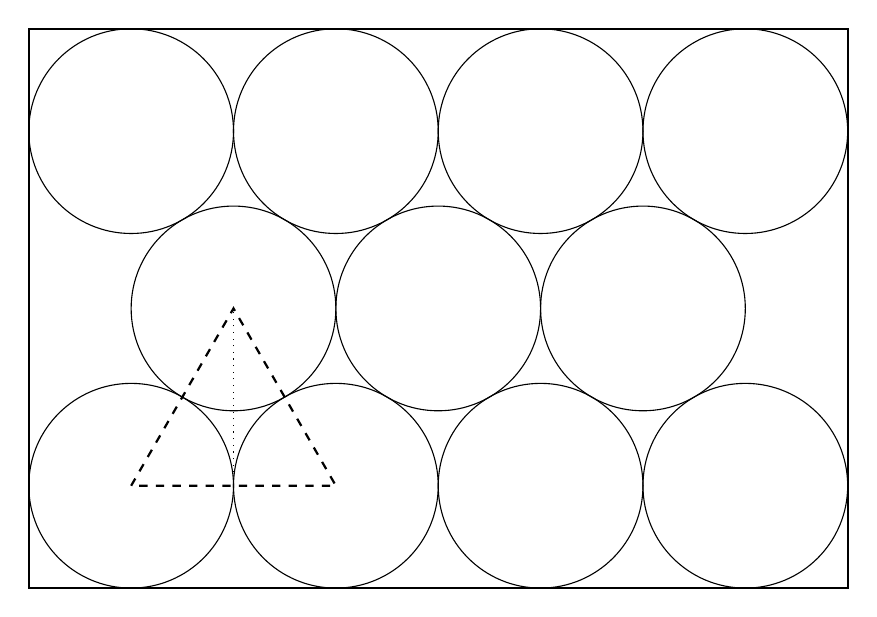
\begin{tikzpicture}[x=.65mm,y=.65mm]
\draw[thick](0,0)rectangle(160,109.282);
\foreach\x in{20,60,100,140}{\draw(\x,20)circle(20);\draw(\x,89.282)circle(20);}
\foreach\x in{40,80,120}{\draw(\x,54.641)circle(20);}
\draw[thick,dashed](20,20)--(40,54.641)--(60,20)--cycle;
\draw[dotted](40,20)--(40,54.641);
\end{tikzpicture}\end{center}
\textbf{Hints.} First lock a complete row of four against the width. Ask where a disk in the next row can nestle most deeply. Then compare its center triangle with the equal-sided triangle from the ring proof. A child explaining that 11 failed in one arrangement has not proved every arrangement impossible. The printed row restriction gives a precise, worthwhile statement they \emph{can} prove. No claim is made here about arbitrary 11-disk packings in 108 mm, or about infinite packing density.
\newpage
\heading{Problems 10--11: optional exact upper bounds}
These are later investigations for children who seek a general size rule; keep concrete maximum-hunting available while a mathematically prepared adult supplies angle comparisons. No K--1 trigonometry or compulsory formula derivation is intended. A concrete answer to Problem 11 can begin with scale: doubling both diameters scales every legal ring, so its maximum count stays the same. Children can investigate the ratio before seeking an exact formula.

For equal outer radius $r$ and middle radius $R$, outer centers lie on radius $R+r$. A chord spanning angle $\theta\le 180^\circ$ has length $2(R+r)\sin(\theta/2)$. Nonoverlap requires at least $2r$, so each successive gap is at least $\alpha=2\arcsin(r/(R+r))$. The total angle is $2\pi$. Conversely, $N=\lfloor 2\pi/\alpha\rfloor$ equally spaced outer disks fit: their smallest pair angle is $2\pi/N\ge\alpha$. This proves the Problem 11 rule for positive radii and an unlimited supply of congruent outside disks. Around the 120 mm middle twelve 40 mm disks fit ($\alpha=2\arcsin(1/4)\approx 28.955^\circ$; thirteen need $376.4^\circ$). The four equal rings give 4, 6, 9 and 12 for middle-to-outside ratios $\tfrac12,1,2,3$. A circumference estimate (centers on a circle of radius $R+r$, each disk using about $2r$ of it) gives $\pi(R/r+1)\approx 4.7, 6.3, 9.4, 12.6$, and the answers are the whole numbers just below. The estimate is never too small, since a chord is shorter than its arc, but it can be one too big: for ratio 2.2 it gives 10.05 while nine fit.

For $(R,r)=(40,20)$, $\alpha\approx 38.942^\circ$: nine fit and ten require $389.42^\circ$. For $(20,40)$, $\alpha\approx 83.621^\circ$: four fit and five require $418.10^\circ$. The same-size case gives 60 degrees and six. An empirical count for a few radii does not establish the formula.

\textbf{Problem 10 without angles.} Slide each outside disk around the middle, keeping contact, until it touches the next one. Each disk moves into empty space, so a legal ring becomes a chain of touching disks with one gap left. Nine small disks chained around the 80 mm middle leave about 9 mm between the first and the last, and four large disks around the 40 mm middle about 18 mm; six equal disks close up exactly. A ten-disk ring would slide into the nine-disk chain with its tenth disk in that 9 mm gap, which is impossible.

For mixed outer radii $a,b$, the least allowed pair angle follows from
\[
\cos\theta\le\frac{(R+a)^2+(R+b)^2-(a+b)^2}{2(R+a)(R+b)}.
\]
Around radius 40: small-small need $\alpha=2\arcsin(1/3)$; large-small need $\beta=\arccos(2/3)\approx 48.190^\circ$; large-large need 60 degrees. Any mixed nine-ring has two gaps incident to a large disk at least $\beta$ and its other seven gaps at least $\alpha$. Their sum $2\beta+7\alpha\approx 368.976^\circ$ exceeds 360. Larger rings are also impossible. The eight-witness on page 3 is checked pairwise.

Around radius 20: small-small need 60 degrees, large-small need $\gamma=\arccos(1/3)\approx 70.529^\circ$, and large-large need $2\arcsin(2/3)>\gamma$. A mixed six-ring needs at least $2\gamma+4\cdot 60\approx 381.058^\circ$. The five-witness attains the bound. These are exact local maxima under the two available sizes and both-size requirement. They do not follow from inserting an average radius into the congruent-outside formula.

\heading{Sources, connections and what to record}
Boyvalenkov, Dodunekov and Musin, \emph{Kissing numbers---a survey}, arXiv:1507.03631, \S1 pp.1--2, supplies the classical definition and planar value. Center proofs, changed-size witnesses and finite trays are independently designed. Earlier Week 1 fitting and Week 26 perimeter use other shapes/questions; this family introduces circular tangency and angular bounds. \emph{Math Circle by the Bay}, Preface viii--x, supports varied pace and substantial hands-on themes; the specific routes here are unpiloted design choices.

Record actual problem IDs, disk/tray sizes and attempted arrangements; distinguish a successful construction, guessed maximum, finite checks and a general explanation. Note whether children checked contacts themselves and any material failure. Do not mark a prepared packet as taught. See source QA for independent review, mathematical checks and clean rebuild evidence; no physical or classroom certification is implied.
\end{document}
